\subsection{Komponen \textit{Resource Controller}}

Seperti yang sudah dirancangkan sebelumnya, kelas ini menggunakan \textit{Kubernetes Client API} untuk mengubah alokasi sumber daya. Diimplementasikan dengan sistem antrian, sehingga jika sejumlah rule aktif secara bersamaan, maka akan dijalankan secara berurutan. Terdapat sebuah fungsi \textit{tick} yang akan berfungsi untuk mengeksekusi antrian. Contoh simpanan file antrian dapat dilihat pada gambar \ref{fig:ex-queue-rc}. File tersebut menyimpan status alokasi sumber daya pada saat itu, kapan melakukan perubahan pada antrian berikutnya dalam waktu UNIX dan antrian yang akan dieksekusi satu per satu.

\begin{figure}[h]
    \centering
    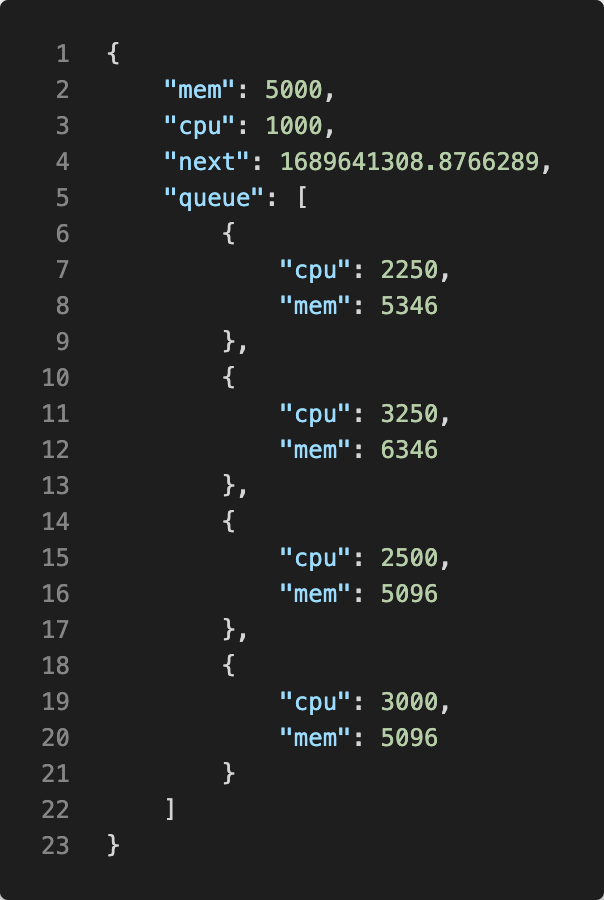
\includegraphics[width=0.45\textwidth]{chapter-4/rc-queue-ex.png}
    \caption{Contoh File Antrian Pengubahan Alokasi}
    \label{fig:ex-queue-rc}
\end{figure}

% TODO CONTOH SISTEM ANTRIAN